\chapter{App}
\begin{figure}[H]
        \centering
        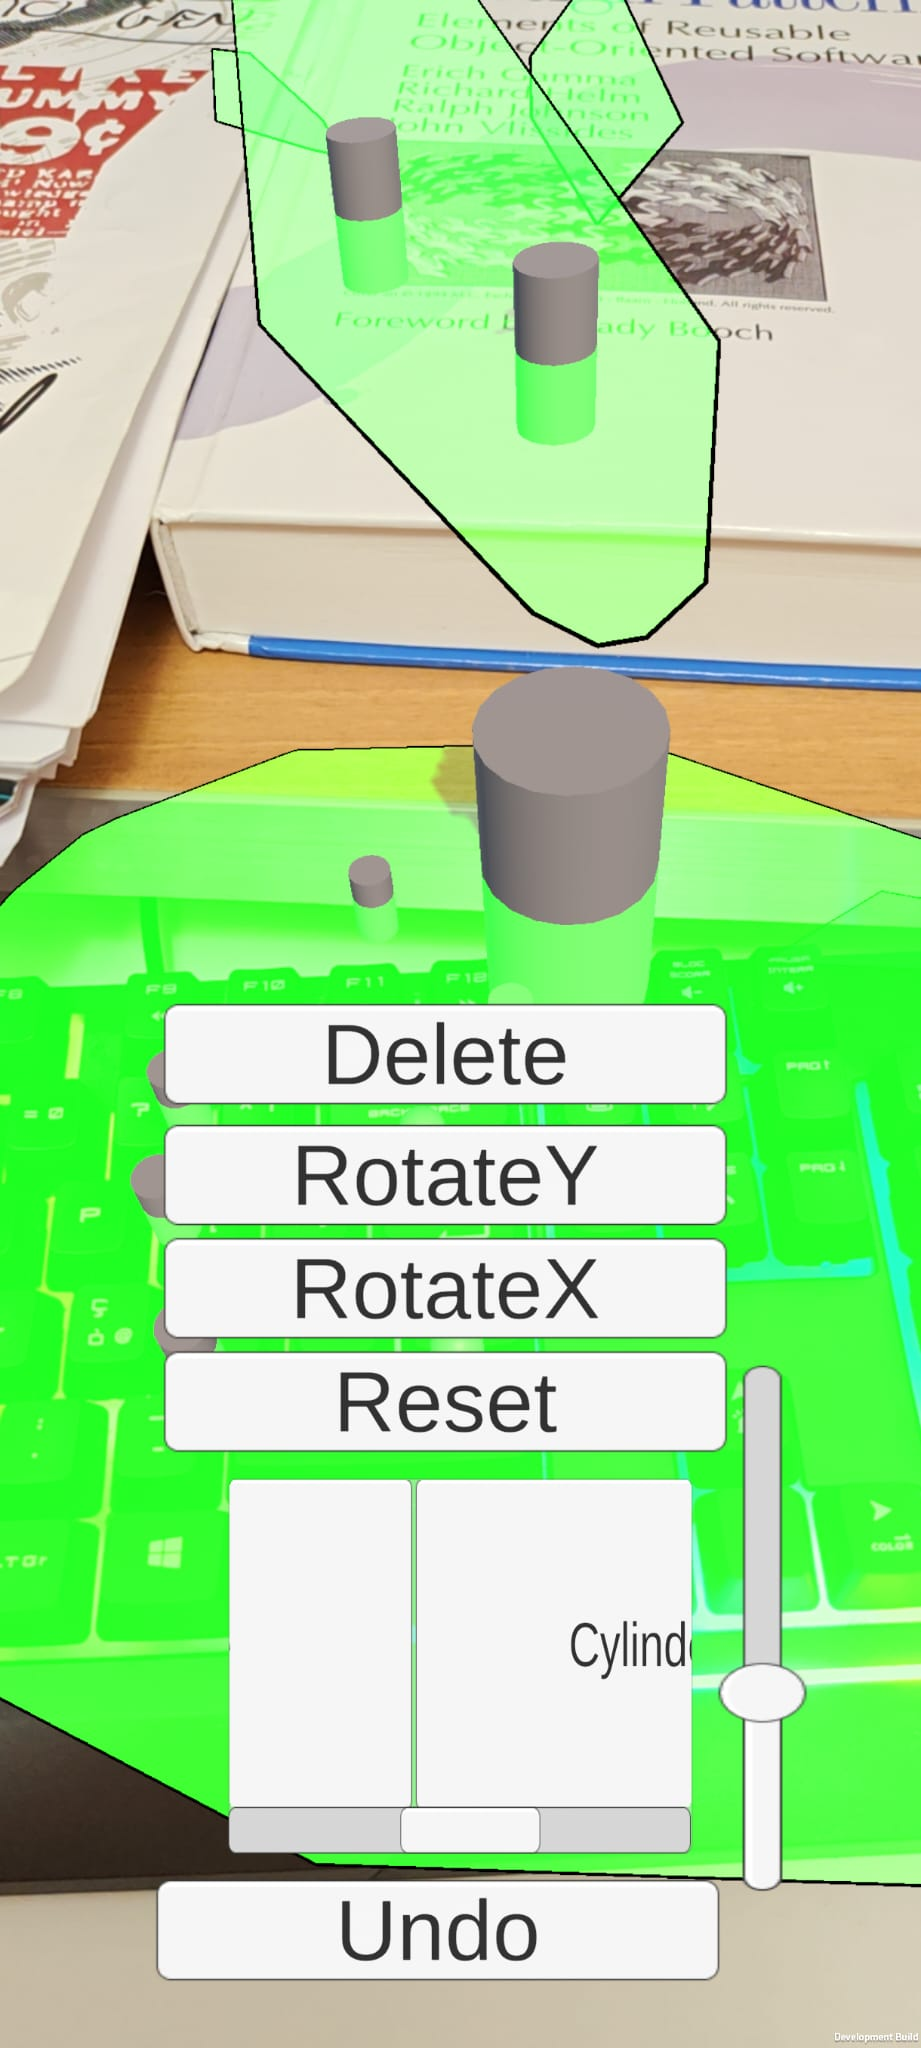
\includegraphics[width=0.4\textwidth]{images/app/MainAppInUseScreen.jpeg} 
        \caption{ Screen while my app is running on my phone}
        \label{fig:dt}
    \end{figure}
    \begin{figure}[H]
        \centering
        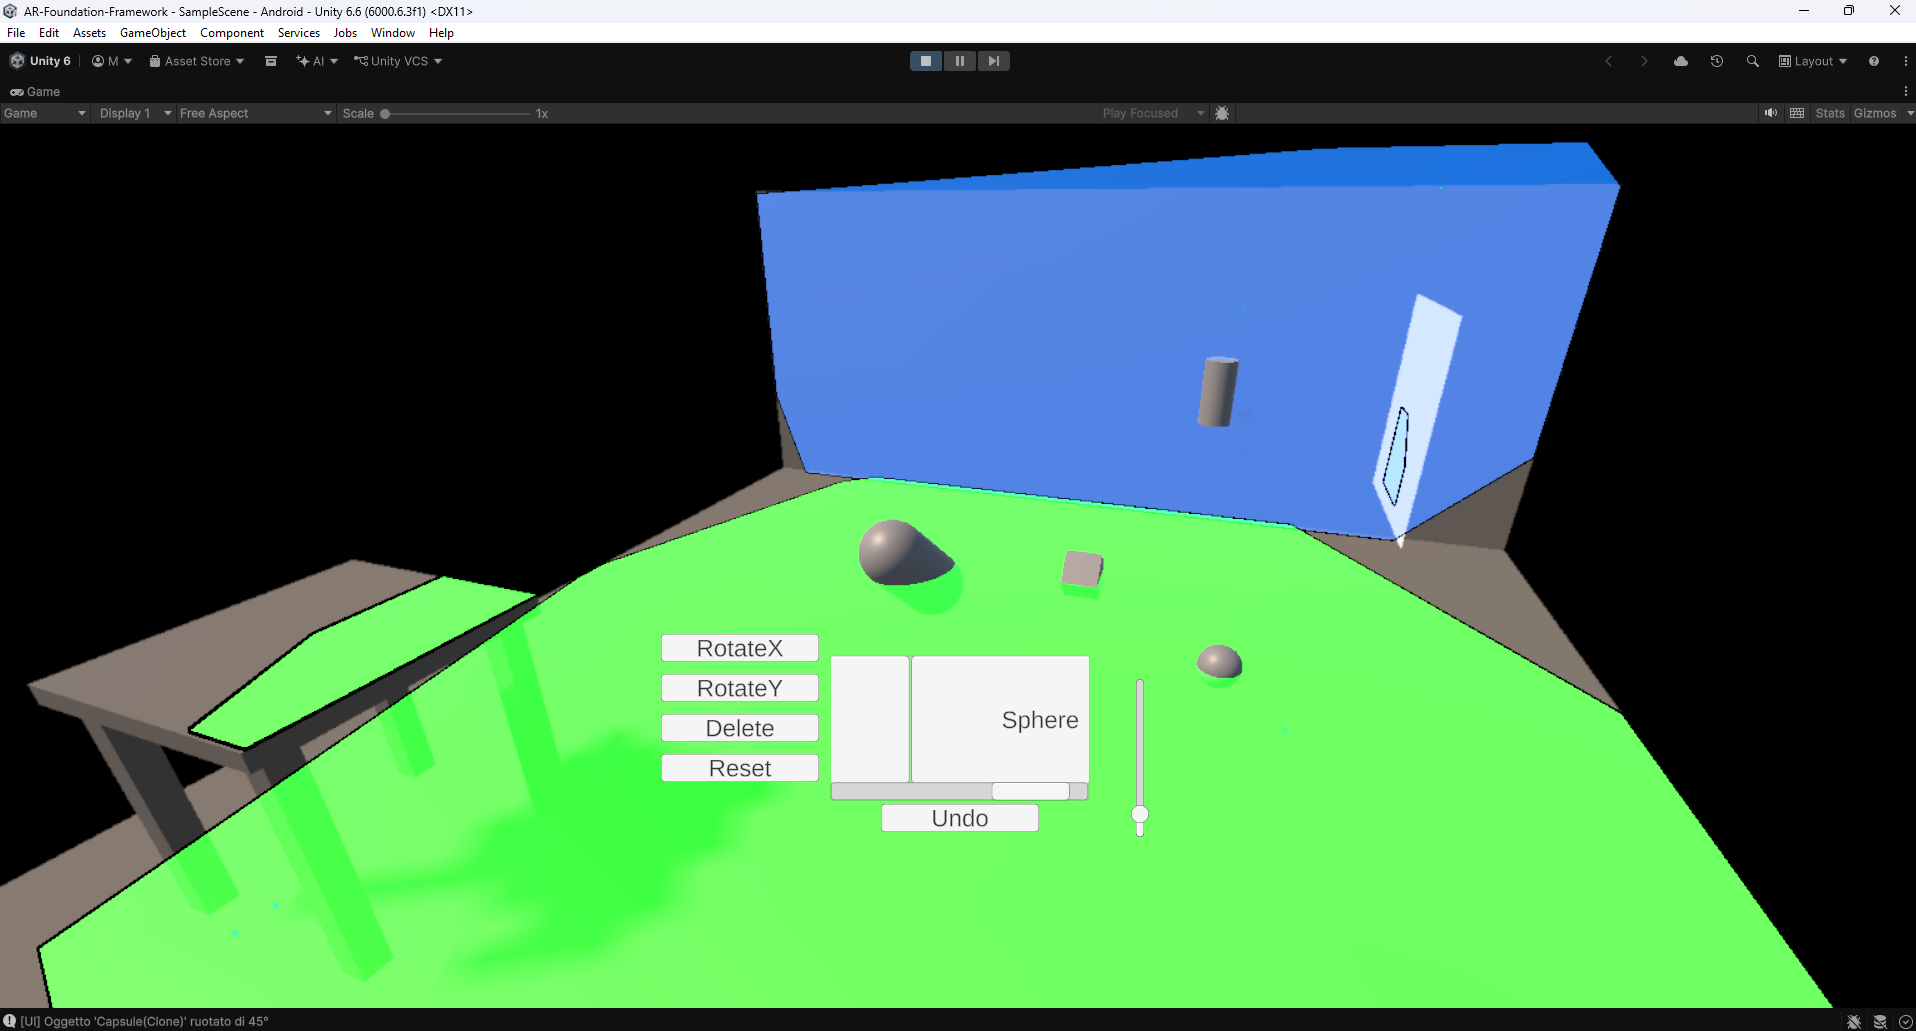
\includegraphics[width=0.7\textwidth]{images/app/AppInUseInEditor.png} 
        \caption{ Screen while my app is running in Unity XR Simulator}
        \label{fig:dt}
    \end{figure}


\section{Analisi Dei Requisiti}

\subsection{Scopo e Uso}
L'applicazione sviluppata in questo progetto è un app AR di tipo Markerless e Video See-Through, la quale consiste nella creazione dinamica di oggetti tridimensionali su superfici piane, con possibilità di eliminare, ruotare, scalare, spostare con drag and drop, pulire la scena e applicare \texttt{"l'undo"} alle azioni dell'utente (annullamento dell'azione), il quale interagisce tramite una semplice GUI composta da pulsanti, slider e per quanto riguarda \texttt{l'XR Simulator} con un input che prevede gestione del click del mouse, di una telecamera virtuale ARCamera e la possibilità di muoversi con WASD con la tastiera nell'editor di Unity e invece per quanto riguarda la distribuzione mobile del touch del touchscreen e della telecamera e sensori del cellulare.

Quest'app è stata distribuita su Android usando ARCore XR Plug-In.
Come si può presumere, l'app distribuita su smartphone avrà un margine d'errore maggiore rispetto all'editor, derivato dal fatto che non si hanno superfici e telecamere/sensori ideali e stabili come nell'editor, infatti ciò può portare ad ulteriori ritardi, errori, saturazione e ha tanti altri fattori negativi. 

Per la realizzazione di tale software, ho fatto uso di 3 manager di AR principali, ovvero \texttt{ARPlane, ARRaycast e ARPointCloud} aggiunti come componenti all'\texttt{XR Origin}, con in aggiunta due manager custom creati da me per personalizzare \texttt{ARPlaneManager e ARPointCloudManager}, facendo in modo, rispettivamente, di vedere tre colori diversi per superfici verticali e orizzontali e quando l'oggetto è in stato di \texttt{"drag"} e stessa cosa per quanto riguarda i \texttt{"point cloud"}, un colore di default e l'altro quando il drag è attivo. Esempio di parte di codice usato per CustomPlaneManger: 
\begin{lstlisting}[language={[Sharp]C}]
public class CustomPlaneManager : MonoBehaviour
{
    //...
     private void OnPlanesChanged(ARTrackablesChangedEventArgs<ARPlane> args)
     {
         foreach (var plane in args.added)
             ApplyDefaultPlaneColor(plane);
         foreach (var plane in args.updated)
         {
             if (plane != currentlyActivePlane)
                 ApplyDefaultPlaneColor(plane);
         }
     }
    private void ApplyDefaultPlaneColor(ARPlane plane)
    {
        if (plane == null) return;
        Color targetColor = plane.alignment switch
        {
            PlaneAlignment.HorizontalUp or PlaneAlignment.HorizontalDown => horizontalColor,
            PlaneAlignment.Vertical => verticalColor,
            _ => defaultColor //_ scelta default
        };
        SetPlaneColor(plane, targetColor);
    }
    private void SetPlaneColor(ARPlane plane, Color color)
    {
        Renderer renderer = plane.GetComponent<Renderer>() ?? plane.GetComponentInChildren<Renderer>();
        if (renderer != null && renderer.material != null)
        {
            renderer.material.color = color;
        }
    }//...
}
\end{lstlisting}


In particolare, i 3 componenti AR usati sono: 
\begin{itemize}

    \item \textbf{ARPointCloudManager} serve a rilevare i "feature points" (punti di interesse), ovvero elementi visivi distintivi (angoli, trame, contrasti) che la fotocamera del dispositivo usa per orientarsi nello spazio; genera una "nuvola di punti" tridimensionale che rappresenta la struttura grezza dell'ambiente circostante e viene utilizzato principalmente dal sistema interno di tracciamento (SLAM) per capire come si muove il dispositivo ed è utile durante lo sviluppo o nelle fasi di calibrazione per mostrare all'utente che il sistema sta effettivamente "vedendo" l'ambiente.
    
    \item \textbf{ARPlaneManager} analizza la nuvola di punti e le immagini della fotocamera per identificare e ricostruire superfici piane reali; riconosce e traccia superfici piatte, classificandole automaticamente in piani orizzontali (es. pavimenti, tavoli), piani verticali (es. pareti, porte) e piani inclinati ed unisce automaticamente piani adiacenti se rileva che fanno parte della stessa superficie e aggiorna i loro confini in tempo reale man mano che l'utente inquadra l'ambiente. 

    \item \textbf{ARRaycastManager} permette di generare dei "raggi" virtuali dallo schermo del dispositivo verso l'ambiente reale per trovare punti di intersezione con gli elementi rilevati; esegue un test di collisione (raycasting) non contro i normali collider di Unity, ma contro i dati AR generati dall'ambiente (superfici tracciate dall'ARPlaneManager o feature points dell'ARPointCloudManager), per questo per il sistema di \texttt{drag and drop} degli oggetti ho fatto uso del raycast fisico che si basa sui collider; è essenziale per l'interazione dell'utente, poichè quando quest'ultimo tocca lo schermo, l'ARRaycastManager determina l'esatto punto nello spazio 3D reale in cui posizionare un oggetto.

\end{itemize}


\subsection{Requisiti Funzionali}

\subsubsection{RF1 - Interfaccia Grafica}
\begin{itemize}
    \item \textbf{RF1.1} - Il sistema deve mostrare i pulsanti che agiscono sull'oggetto, ovvero Delete, CleanAllObject, Rotate(x and y) and Spawn
    \item \textbf{RF1.2} - Il sistema deve mostrare il pulsante per l'annullamento delle azioni
    \item \textbf{RF1.3} - Il sistema deve mostrare una Scroll View per selezionare l'oggetto da spawnare
    \item \textbf{RF1.4} - Il sistema deve mostrare uno Slider per cambiare la scala di un oggetto selezionato a runtime
\end{itemize}

\subsubsection{RF2 - Sistema Di Input}
\begin{itemize}
    \item \textbf{RF2.1} - Il sistema deve avere accesso alla telecamera del dispositivo mobile oppure una camera virtuale di un simulatore
    \item \textbf{RF2.2} - Il sistema deve avere accesso a vari sensori del dispositivo
    \item \textbf{RF2.3} - Il sistema deve consentire all'utente di interagire tramite il touch da mobile (il movimento con WASD qua è camminare nel mondo reale) e con il mouse e tastiera(WASD) dal simulatore.
\end{itemize}

\subsubsection{RF3 - Sistema Di Output e Comportamento}
\begin{itemize}
    \item \textbf{RF3.1} - Il sistema deve poter intercettare e visualizzare a schermo le superfici piane(verticali, orizzontali o inclinati), in corrispondenza con il mondo reale
    \item \textbf{RF3.2} - Il sistema deve poter intercettare e visualizzare a schermo le varie point clouds, in corrispondenza con il mondo reale 
    \item \textbf{RF3.3} - Il sistema deve poter interpretare e capire quando vede un piano tramite operazione di Raycast
\end{itemize}

\subsection{Requisiti Non Funzionali}
\subsubsection{RNF1 – Usabilità}

\begin{itemize}
  \item \textbf{RNF1.1} - I comandi devono essere intuitivi e facilmente accessibili
    (\texttt{WASD}/frecce, mouse, pulsanti, scroll view, slider).
  \item RNF1.2 - L'interfaccia deve essere chiara e mostrare informazioni essenziali
    (comandi e output).
  \item RNF1.3 - Il sistema deve essere comprensibile senza necessità di un tutorial complesso.
\end{itemize}

\subsubsection{RNF2 – Affidabilità}  Il sistema non deve andare in crash durante una sessione di uso standard.


\subsubsection{RNF3 – Manutenibilità}
\begin{itemize}
  \item RNF3.1 - Il codice deve essere strutturato in moduli separati.
  \item RNF3.2 - Il sistema deve permettere l'aggiunta di nuovi prefab o nuove funzioni senza
    modificare pesantemente il codice esistente.
\end{itemize}

\subsubsection{RNF4 – Portabilità}

\begin{itemize}
  \item RNF4.1 - Il sistema deve essere eseguibile sui sistemi operativi scelti.
  \item RNF4.2 - Il sistema non deve dipendere da librerie non portabili o non supportate.
\end{itemize}

\subsubsection{RNF5 – Sicurezza}  Il sistema deve impedire input non validi o fuori dai limiti


\subsubsection{RNF6 – Qualità grafica} Gli asset grafici devono essere leggibili e non confondere l'utente.


\subsubsection{RNF7 – Scalabilità} Il sistema deve poter gestire l'aggiunta di ulteriori elementi senza degradare significativamente le prestazioni.

\section{Design Pattern}
\subsection{Convenzioni di Nomenclatura}

\begin{itemize}
  \item Le \textbf{classi astratte} sono prefissate con \texttt{A}.
  \item Le \textbf{interfacce} sono prefissate con \texttt{I}.
  \item I \textbf{metodi} e le \textbf{classi concrete} seguono \textit{QuestoCase}.
  \item Le \textbf{variabili} sono tutte minuscole con separatore \texttt{\_}.
  \item Le \textbf{variabili con Setter e Getter} sono tutte con l'iniziale maiuscola con separatore \texttt{\_}.
  \item le variabili evento observer Action (\textbf{eventi observer Action}) dell'engine sono con una sola iniziale maiuscola (obbligatorio) e il resto in minuscolo con separatore \texttt{\_}.
\end{itemize}

\subsection{Command}
Design pattern comportamentale e consente di incapsulare un'azione dentro ad un oggetto, diasaccopiando chi invoca l'azione da chi la esegue.
Nel progetto è stato usato per le azioni che può compiere l'utente, integrando anche il meccanismo di annullamento dell'azione (undo).
(Vedi in Factory Method per l'implementazione di un comando)
\begin{lstlisting}[language={[Sharp]C}]
public interface ICommand
{
    void Execute();
    void Undo();
}
\end{lstlisting}

\subsection{State}
Design pattern comportamentale e consente ad un oggetto di cambiare il proprio comportamento a runtime in base allo stato in cui si trova e quindi di cambiare anche quest'ultimo. Nel progetto è stato usato per rappresentare i vari stati diversi dell'interazione con gli oggetti.

\begin{lstlisting}[language={[Sharp]C}]
public interface IObjectInteractionState
{
    void EnterState(ARMainApplication context, GameObject obj);
    void UpdateState(ARMainApplication context, GameObject obj);
    void ExitState(ARMainApplication context, GameObject obj);
}

public class SpawnState : IObjectInteractionState
{
    public void EnterState(ARMainApplication context, GameObject obj)
    {
        if (context.Object_Factory != null && context.Hit_List.Count > 0)
        {
            Pose hit_pose = context.Hit_List[0].pose;
            SpawnContext spawn_context = new SpawnContext(
                hit_pose,
                context.Object_To_Spawn,
                context.Objects_Spawned,
                context.Load_Prefabs.Spawnable_Objects,
                context.Main_Camera
            );

            // Invece di chiamare direttamente lo Spawn, incapsuliamo nel Command
            ICommand spawn_cmd = new SpawnObjectCommand(context.Object_Factory, spawn_context, context);
            context.ExecuteCommand(spawn_cmd);
        }

        context.ChangeState(new IdleState(), null);
    }

    public void UpdateState(ARMainApplication context, GameObject obj) { }
    public void ExitState(ARMainApplication context, GameObject obj) { }
}
public class ARMainApplication : MonoBehaviour
{
    //...
    public void ChangeState(IObjectInteractionState newState, GameObject targetObj)
    {
        current_state?.ExitState(this, targetObj);
        current_state = newState;
        current_state?.EnterState(this, targetObj);
    }
    //...
}
\end{lstlisting}

\subsection{Observer}
Design pattern comportamentale che definisce come gli oggetti comunicano quando uno cambia stato, notificando automaticamente tutti gli osservatori (Per Invoke guarda Factory Method).
Nel progetto è stato usato per condividere informazioni sugli stati dell’applicazione, come la modalità di trascinamento (dragging) o lo spawn di un nuovo oggetto, senza che le classi coinvolte si conoscano direttamente.

L’implementazione sfrutta i delegate di C\#: ARMainApplication espone eventi di tipo Action (ad esempio On\_dragging\_state\_changed), a cui gli altri componenti si iscrivono con l’operatore +=. La parola chiave event impedisce agli iscritti di invocare l’evento o di sovrascrivere gli altri osservatori, mantenendo l’incapsulamento. Quando lo stato cambia, il setter della proprietà richiama Invoke tramite l’operatore ?., che evita errori se nessun osservatore è iscritto. La notifica avviene solo se il valore è effettivamente cambiato, evitando chiamate inutili. In questo modo ARMainApplication (il subject) rimane disaccoppiato dagli osservatori, che possono essere aggiunti o rimossi senza modificarlo.

\begin{lstlisting}[language={[Sharp]C}]
public class ARMainApplication : MonoBehaviour
{
    public event Action<bool> On_dragging_state_changed;
    //...
     public bool Is_Dragging
     {
         get => is_dragging;
         set
         {
             if (is_dragging != value)
             {
                 is_dragging = value;
                 On_dragging_state_changed?.Invoke(is_dragging); // Notifica Observer
             }
         }
     }
     //...
    public void NotifyObjectSpawned(GameObject spawnedObj)
   {
       On_object_spawned?.Invoke(spawnedObj);
   }

}

\end{lstlisting}

\subsection{Factory Method}
Design Pattern creazionale che consente di creare oggetti senza specificare esplicitamente la loro classe concreta, delegando la creazione alle sottoclassi. Nel progetto è stato usato per la creazione di oggetti.
\begin{lstlisting}[language={[Sharp]C}]
public abstract class ASpawnObjectFactory
{
    public abstract GameObject SpawnObject(SpawnContext context);
}

public class SpawnObjectCommand : ICommand
{
    private readonly ASpawnObjectFactory factory;
    private readonly SpawnContext spawn_context;
    private readonly ARMainApplication ar_app;
    private GameObject spawned_object;

    public SpawnObjectCommand(ASpawnObjectFactory factory, SpawnContext spawn_context, ARMainApplication ar_app)
    {
        this.factory = factory;
        this.spawn_context = spawn_context;
        this.ar_app = ar_app;
    }

    public void Execute()
    {
        spawned_object = factory.SpawnObject(spawn_context);
        if (spawned_object != null && ar_app != null)
        {
            ar_app.NotifyObjectSpawned(spawned_object);
        }
    }

    public void Undo()
    {
        if (spawned_object != null)
        {
            if (ar_app != null && ar_app.Objects_Spawned.Contains(spawned_object))
            {
                ar_app.Objects_Spawned.Remove(spawned_object);
            }
            Object.Destroy(spawned_object);
        }
    }
}
\end{lstlisting}



\subsection{Struttura Dati: CommandHistory}
è una struttura dati, creata da me, formata da una \texttt{LinkedList} di \texttt{ICommand}, implementato come uno stack, in modo da creare il meccanismo di \texttt{undo} ed eliminare l'undo o dei comandi per oggetti selezionabili che possono non coincidere con gli ultimi inseriti. 
\begin{lstlisting}[language={[Sharp]C}]
public class CommandHistory
{
    private readonly LinkedList<ICommand> history = new LinkedList<ICommand>();
    private readonly int maxCapacity;

    public CommandHistory(int maxCapacity = 10)
    {
        this.maxCapacity = maxCapacity;
    }

    public void Push(ICommand command)
    {
        history.AddLast(command);

        // Se superiamo la capacita' massima, rimuoviamo il primo elemento (il piu' vecchio)
        if (history.Count > maxCapacity)
        {
            ICommand oldestCommand = history.First.Value;
            history.RemoveFirst();

            // Se il comando eliminato e' una cancellazione definitiva, puliamo la risorsa
            if (oldestCommand is DeleteObjectCommand deleteCmd)
            {
                deleteCmd.DisposeAndDestroyPermanent();
            }
        }
    }

    public ICommand Pop()
    {
        if (history.Count == 0) return null;

        ICommand lastCommand = history.Last.Value;
        history.RemoveLast();
        return lastCommand;
    }

    public int Count => history.Count;

    //Serve in DeleteObjectCommand, poiche' l'oggetto selezionato puo' essere diverso dall'ultimo messo
    public bool RemoveCommand(ICommand command)
    {
        if (command == null) return false;

        LinkedListNode<ICommand> node = history.Find(command);
        if (node != null)
        {
            history.Remove(node);
            Debug.Log("[CommandHistory] Comando rimosso con successo dallo storico!");
            return true;
        }
        Debug.LogWarning("[CommandHistory] Impossibile trovare il comando da rimuovere nello storico.");
        return false;
    }
}
\end{lstlisting}

\section{Analisi delle Prestazioni e Profiling}

Per la valutazione sperimentale e l'ottimizzazione dell'applicazione è stato impiegato il \textit{Unity Profiler}\cite{profiler}, strumento di diagnostica integrato nell'engine che monitora in tempo reale e con frequenza al frame (un \textit{frame} è ciascuna immagine prodotta e mostrata a schermo) il carico computazionale sulla CPU, l'occupazione della memoria (RAM e \textit{Managed Heap}) e l'efficienza della pipeline di rendering. Il suo scopo è isolare i colli di bottiglia (\textit{bottlenecks}) e stabilire se i rallentamenti siano imputabili all'elaborazione logica, alle chiamate di disegno verso la GPU o alla gestione delle risorse di memoria.

\begin{figure}[H]
        \centering
        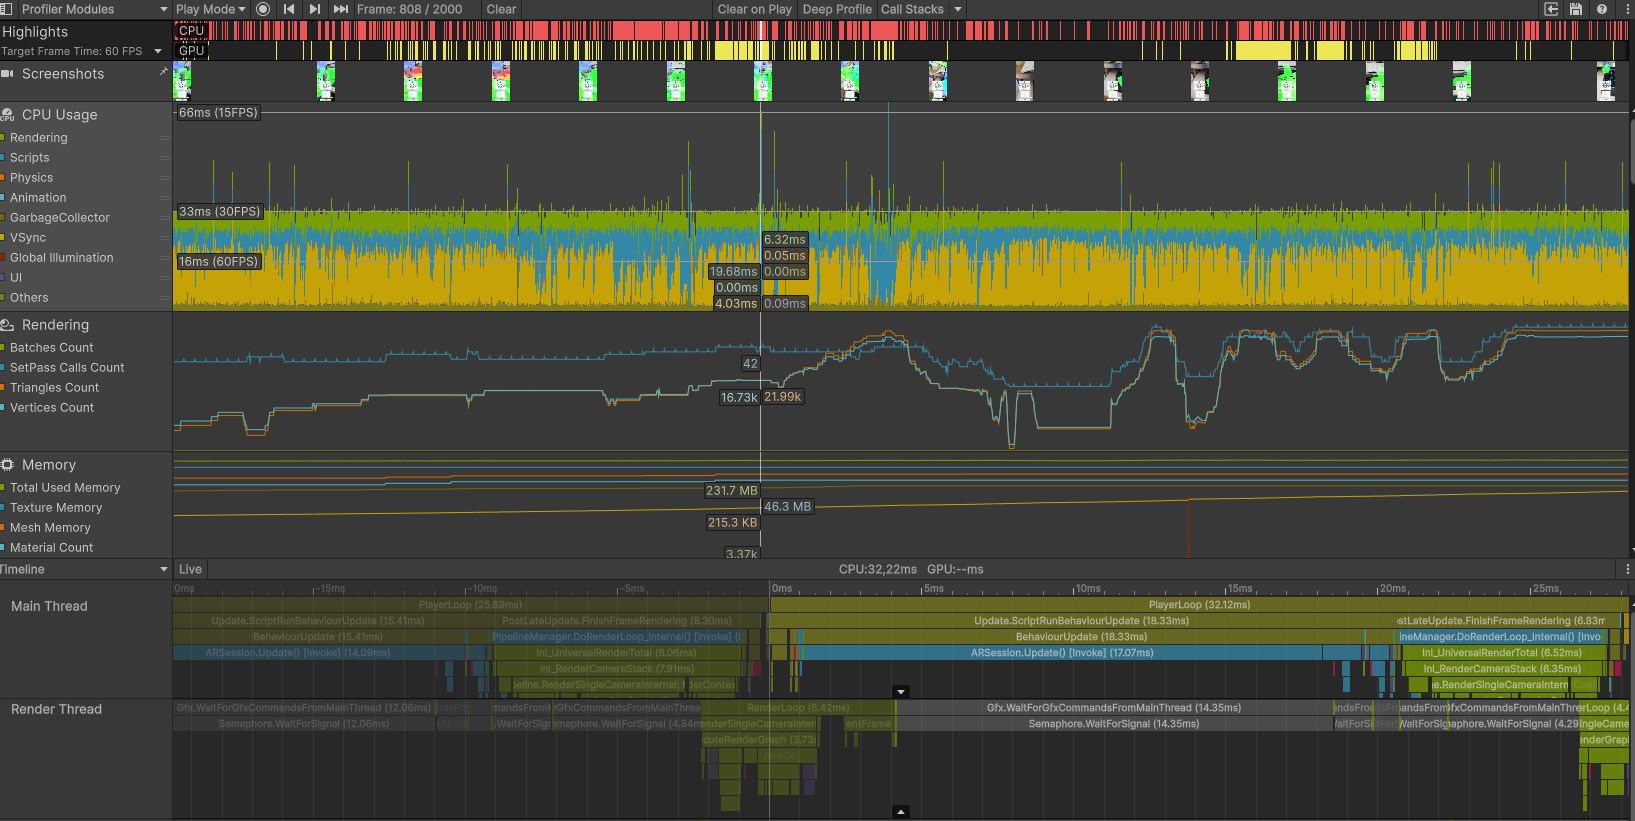
\includegraphics[width=0.7\textwidth]{images/app/GeneralStat.png} 
        \caption{Schermata generale dell'Unity Profiler durante l'esecuzione dell'applicazione sul dispositivo di test.}
        \label{fig:generalstat}
\end{figure}

I test sono stati condotti \textit{on-device} (direttamente sul dispositivo fisico e non nell'Editor di Unity), tramite build di debug collegata via ADB (\textit{Android Debug Bridge}, strumento di comunicazione tra computer e dispositivo Android) ad un dispositivo di fascia medio-alta, un \textbf{Motorola Edge 70} con:
\begin{itemize}
\item \textbf{Sistema Operativo:} Android 16.
\item \textbf{SoC e CPU:} Qualcomm Snapdragon 7 Gen 4 (\textit{SoC}, \textit{System on Chip}: unico chip che integra CPU, GPU ($1.15\text{ GHz}$) e altri componenti), Octa-Core, con clock fino a $2.8\text{ GHz}$.
\item \textbf{GPU:} Adreno 722.
\item \textbf{RAM:} $12\text{ GB}$ LPDDR5X (memoria RAM per dispositivi mobili, a basso consumo).
\item \textbf{Sensori coinvolti nel tracciamento:} fotocamera, accelerometro, giroscopio e magnetometro, con un Sensor Hub dedicato (coprocessore a basso consumo che raccoglie i dati dei sensori) per la fusione dei dati di tracciamento \textit{spatially-aware} (consapevole della posizione e dell'orientamento del dispositivo nello spazio).
\end{itemize}

\subsection{Tipologie di Grafici e Metodologia di Lettura}

Il profiler organizza la diagnostica in quattro tipologie di grafici, a diversi livelli di astrazione (dall'andamento temporale macroscopico al singolo microsecondo di esecuzione):

\begin{enumerate}
\item \textbf{Grafico ad Area Impilata (\textit{Timeline Stacked Area Chart}):} presente nel modulo \textit{CPU Usage}. Sull'asse $x$ sono riportati i frame sequenziali, sull'asse $y$ il tempo di esecuzione in $\text{ms}$. Le macro-categorie sono aree cromatiche sovrapposte: \textit{Scripts} (codice C\# eseguito, compreso quello dei package come AR Foundation, che nel frame analizzato ne costituisce la parte prevalente.), \textit{Rendering} (preparazione dei comandi grafici da parte della CPU), \textit{Garbage Collector} (meccanismo che libera automaticamente la memoria degli oggetti C\# non più usati, sospendendo temporaneamente il codice), \textit{Physics} (simulazione fisica), \textit{VSync} (attesa della sincronizzazione con l'aggiornamento del display) e \textit{UI} (interfaccia utente). Le linee orizzontali a $16\text{ ms}$ ($60\text{ FPS}$) e $33\text{ ms}$ ($30\text{ FPS}$) permettono di vedere il superamento della soglia del frame e l'impatto di ciascun sottosistema.

\item \textbf{Grafico a Linee (\textit{Line Chart}):} usato nei moduli \textit{Rendering} e \textit{Memory}, mostra l'andamento nel tempo di conteggi e quantità (ad esempio batch, triangoli, memoria usata) frame per frame.

\item \textbf{Traccia di Esecuzione e Threading (\textit{Flame Graph / Call Stack Timeline}):} nella sezione inferiore del profiler è una traccia a blocchi gerarchici annidati analoga a un diagramma di Gantt. Mostra due thread: il \textit{Main Thread} (thread principale, che esegue logica, script e preparazione dei comandi grafici) e il \textit{Render Thread} (thread dedicato che traduce tali comandi in chiamate alla GPU). L'asse orizzontale misura la cronologia interna del singolo frame (in $\text{ms}$), mentre le righe mostrano le chiamate a funzione e l'esecuzione parallela sui thread, evidenziando stalli e sincronizzazioni (\texttt{WaitForGfx\allowbreak Commands}, \texttt{Semaphore.\allowbreak WaitForSignal}).

\item \textbf{Grafici a Barre e Distribuzione Statistica (\textit{Breakdown Bar Charts e Highlights}):} usati in \textit{Selection Highlights}, \textit{Capture Highlights} e \textit{Memory Breakdown}. Barre orizzontali proporzionali mostrano valore assoluto e percentuale delle risorse, con indicatori statistici (minimo, mediana, massimo) per valutare la stabilità della sessione. La mediana è il valore centrale: metà dei frame è più veloce e metà più lenta.
\end{enumerate}

\subsection{Testing}
La cattura analizzata comprende $2000$ frame. Il frame time minimo è $19.198\text{ ms}$, quindi nessun frame rispetta il budget di $16.67\text{ ms}$ richiesto da un target di $60\text{ FPS}$, e la mediana è $33.408\text{ ms}$ (circa $30\text{ FPS}$). Il carico risulta più spesso limitato dalla CPU che dalla GPU (\textit{CPU-bound}, cioè una condizione in cui la velocità di generazione dei frame è limitata dal tempo impiegato dal processore per eseguire il codice e preparare i dati), ma, come mostrano i dati aggregati (\textit{Capture Highlights}), una parte rilevante del tempo di frame è attesa di sincronizzazione e non lavoro computazionale. Le analisi di dettaglio sono state svolte sul frame $808$, scelto perché il suo tempo di CPU ($32.782\text{ ms}$) è prossimo alla mediana della cattura ($33.408\text{ ms}$) e quindi rappresentativo della condizione tipica.

\subsubsection{Analisi del Frame Selezionato}

\paragraph{CPU Usage e profilo temporale.} Il modulo \textit{CPU Usage} misura il tempo necessario alla CPU per completare le operazioni di ciascun frame. A fronte di un target di $60\text{ FPS}$ (budget $\le 16.67\text{ ms}$), l'andamento supera costantemente tale soglia, posizionandosi spesso attorno ai $33\text{ ms}$ ($30\text{ FPS}$). Tale valore può essere influenzato anche da un limite alla frequenza di aggiornamento (\texttt{Application.\allowbreak targetFrameRate}, VSync o cadenza del flusso video di ARCore, la piattaforma Google per la realtà aumentata su Android su cui poggia AR Foundation) e non dipendere solo dal sovraccarico della CPU. La traccia del \textit{Main Thread} nel frame $808$ è così ripartita:

\begin{center}
\small
\begin{tabular}{|p{4.4cm}|p{6.8cm}|p{2.6cm}|}
\hline
\textbf{Routine} & \textbf{Funzione} & \textbf{Durata} \\
\hline
\texttt{Update.\allowbreak ScriptRun\allowbreak Behaviour\allowbreak Update} & Invoca il metodo \texttt{Update()} (eseguito una volta per frame) di tutti i \texttt{MonoBehaviour} attivi, cioè gli script Unity: punto d'ingresso del codice C\# e core della logica. Include le routine della riga seguente. & $18.33\text{ ms}$ \\
\hline
\texttt{ARSession.\allowbreak Update()}, \texttt{ARCameraManager.\allowbreak Update()} & Routine di AR Foundation (livello di Unity che unifica le piattaforme AR, qui basato su ARCore): sincronizzano e analizzano i dati di tracciamento (\textit{feature points}, cioè punti caratteristici dell'immagine usati per stimare la posa del dispositivo, piani rilevati) e convertono i frame video della fotocamera. & fino a $17.07\text{ ms}$ \\
\hline
\texttt{PostLate\allowbreak Update.\allowbreak Finish\allowbreak Frame\allowbreak Rendering} & Il \textit{Main Thread} impacchetta i comandi grafici e li inoltra alla coda del \textit{Render Thread}. & $6.83\text{ ms}$ \\
\hline
\texttt{Gfx.WaitForGfx\allowbreak Commands\allowbreak From\allowbreak MainThread}, \texttt{Semaphore.\allowbreak WaitFor\allowbreak Signal} (\textit{Render Thread}) & Il \textit{Render Thread} attende inattivo che il \textit{Main Thread} termini il frame; il semaforo è un meccanismo di sincronizzazione a basso livello tra thread. & $14.35\text{ ms}$ \\
\hline
\end{tabular}
\end{center}

Le durate sono \textit{inclusive} e annidate: \texttt{ARSession.Update()} viene eseguita all'interno di \texttt{BehaviourUpdate}, quindi i valori non vanno sommati. Ne deriva che la quasi totalità del tempo speso negli \texttt{Update()} ($17.07$ su $18.33\text{ ms}$) è dovuta ad AR Foundation e non agli script applicativi. Le attese del \textit{Render Thread} confermano che esso resta in attesa del completamento dei calcoli sul \textit{Main Thread}.

\paragraph{Rendering e complessità geometrica.} 

\begin{figure}[H]
        \centering
        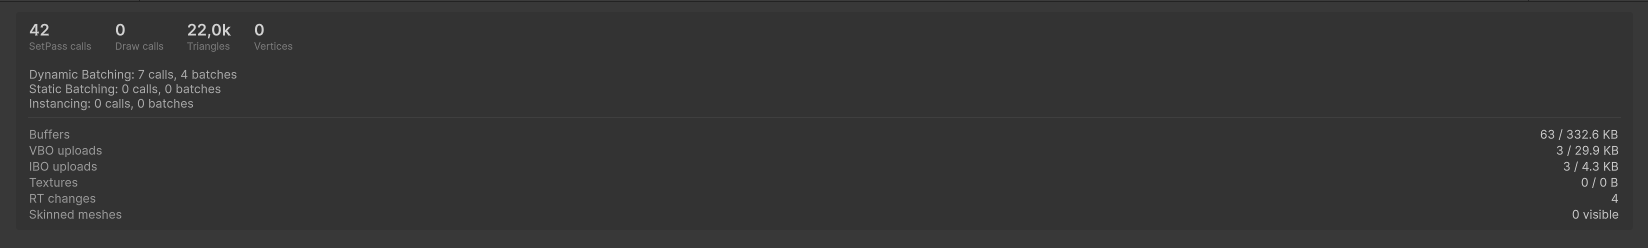
\includegraphics[width=0.8\textwidth]{images/app/RenderingStat.png} 
        \caption{Scheda \textit{Rendering} dell'Unity Profiler.}
        \label{fig:highlightsselection}
\end{figure}

Dai dati del modulo \textit{Rendering} il carico grafico risulta contenuto e non rappresenta il principale collo di bottiglia. Il \textit{Frame Debugger} (strumento che mostra frame per frame la sequenza dei comandi grafici inviati alla GPU) è raggiungibile dallo stesso modulo. I \textit{SetPass Calls}, cioè i cambi di stato di rendering (shader, texture, blending) che comportano un overhead per la CPU, sono $42$, valore molto contenuto per un dispositivo mobile. Il batching dinamico (tecnica che unisce oggetti semplici in un unico gruppo da disegnare, detto \textit{batch}) ha raggruppato $7$ chiamate di disegno in $4$ batch. La \textit{Universal Render Pipeline} (URP) adotta inoltre l'\textit{SRP Batcher}, meccanismo distinto dal batching dinamico che riduce il costo CPU dei cambi di materiale. La geometria conta $22.0\text{k}$ triangoli e $16.73\text{k}$ vertici, cifre che escludono problemi di saturazione della banda di memoria o di geometria eccessiva. Il \textit{GPU Time} non è disponibile per il frame selezionato (\textit{No Value}): la valutazione del carico grafico si basa quindi sulle statistiche di rendering e non su una misura diretta del tempo di GPU.

\paragraph{Memory e Managed Heap.} 
\begin{figure}[H]
        \centering
        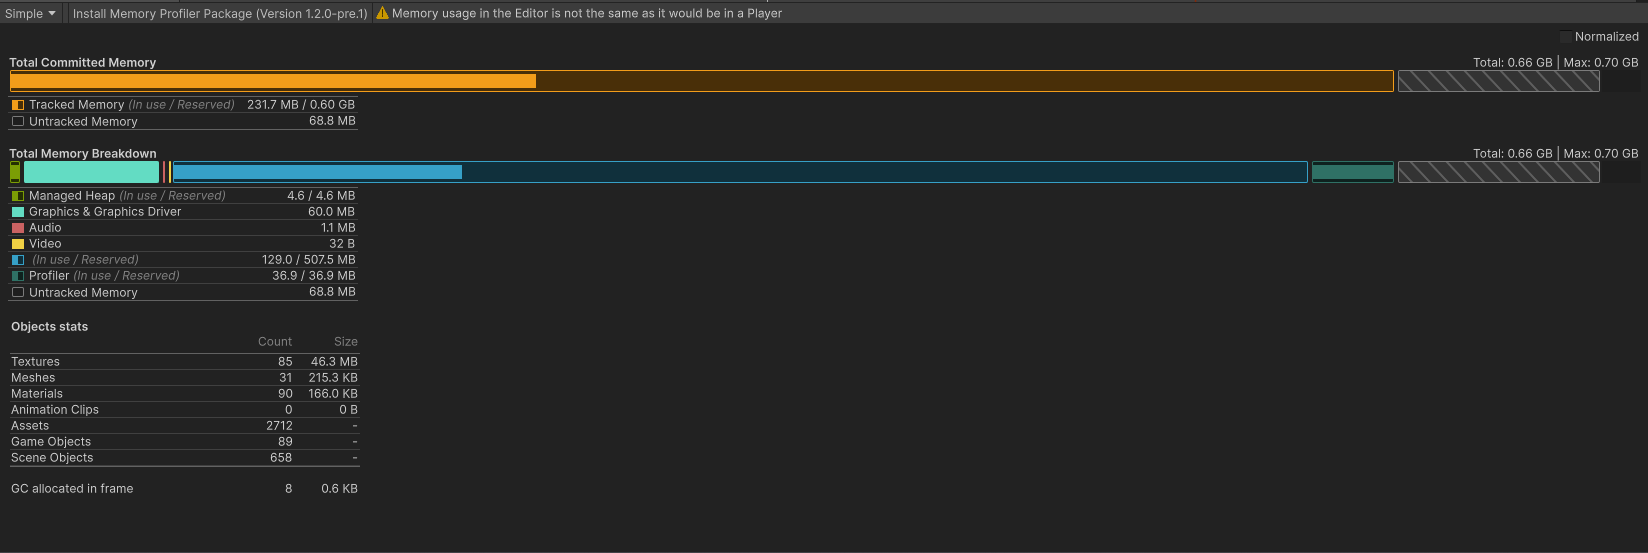
\includegraphics[width=0.8\textwidth]{images/app/MemoryStat.png} 
        \caption{Scheda \textit{Rendering} dell'Unity Profiler.}
        \label{fig:highlightsselection}
\end{figure}

Il modulo distingue la memoria nativa di Unity (C++) dal \textit{Managed Heap}, l'area di memoria in cui vengono allocati gli oggetti C\# e la cui liberazione è affidata al \textit{Garbage Collector} (GC) invece che al programmatore. I consumi globali sono ben controllati, ma critici nelle allocazioni temporanee:
\begin{itemize}
\item \textbf{Total Committed Memory:} $0.66\text{ GB}$ su un massimo di $0.70\text{ GB}$. Indica la memoria complessivamente impegnata dall'applicazione, cioè richiesta al sistema operativo.
\item \textbf{Tracked Memory:} $231.7\text{ MB}$ in uso su $0.60\text{ GB}$ riservati. È la memoria che Unity sa attribuire a oggetti e sistemi; \textit{reserved} indica lo spazio già ottenuto dal sistema operativo, anche se non ancora in uso. A questa si aggiungono $68.8\text{ MB}$ di \textit{Untracked Memory}, non attribuibili da Unity (ad esempio plugin nativi e driver).
\item \textbf{Texture e Mesh:} $46.3\text{ MB}$ per $85$ texture (immagini applicate alle superfici); $215.3\text{ KB}$ per $31$ mesh (modelli geometrici 3D).
\item \textbf{Managed Heap e Garbage Collection:} $4.6\text{ MB}$ in uso, ma con allocazioni continue ad ogni frame: nel frame selezionato $9$ allocazioni per $0.7\text{ KB}$ (\textit{GC Alloc}), originate principalmente da \texttt{Draw AR Background} ($376\text{ B}$) e dal \textit{Render Graph} ($128\text{ B}$); sull'intera cattura le allocazioni sono $18.119$, con un massimo di $43.9\text{ KB}$ in un singolo frame (frame $1396$) e routine di AR Foundation tra i principali contributori. Il valore istantaneo è ridotto, ma l'accumulo genera frequenti interventi bloccanti del GC, che sospende l'esecuzione del codice C\# per ripulire la memoria non più utilizzata.
\end{itemize}

\subsubsection{Analisi Statistica degli Highlights (Selection e Capture)}
\begin{figure}[H]
        \centering
        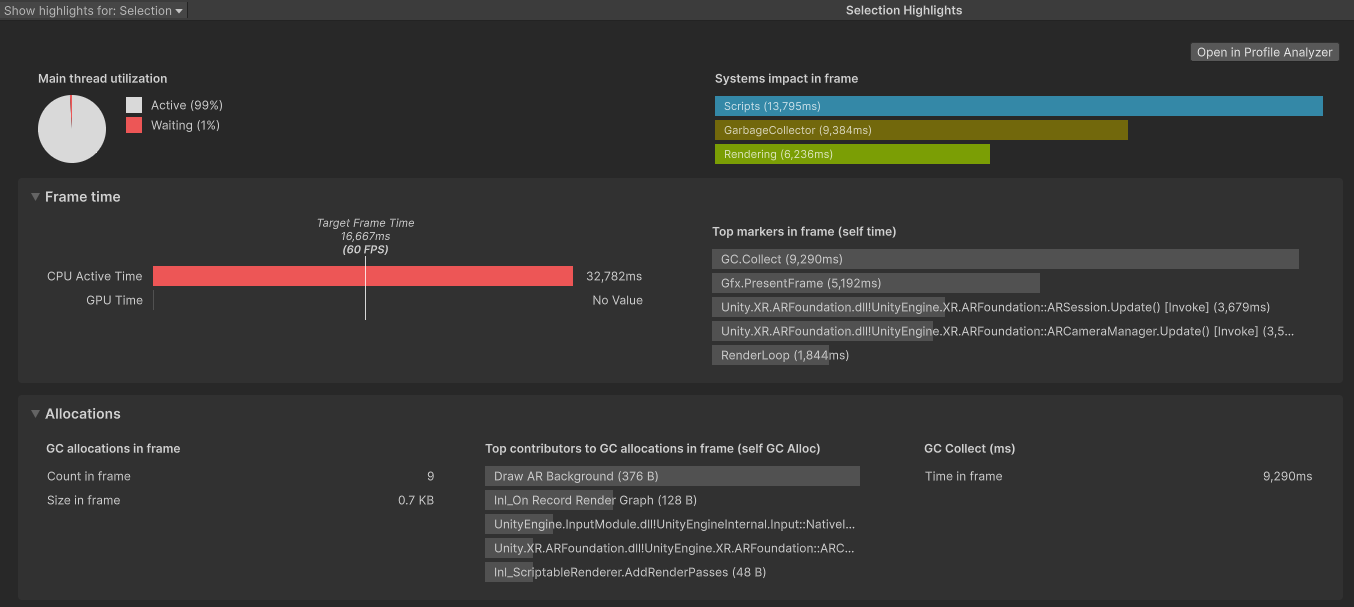
\includegraphics[width=0.7\textwidth]{images/app/HighLightsSelection.png} 
        \caption{Scheda \textit{Selection Highlights} dell'Unity Profiler.}
        \label{fig:highlightsselection}
\end{figure}
\begin{figure}[H]
        \centering
        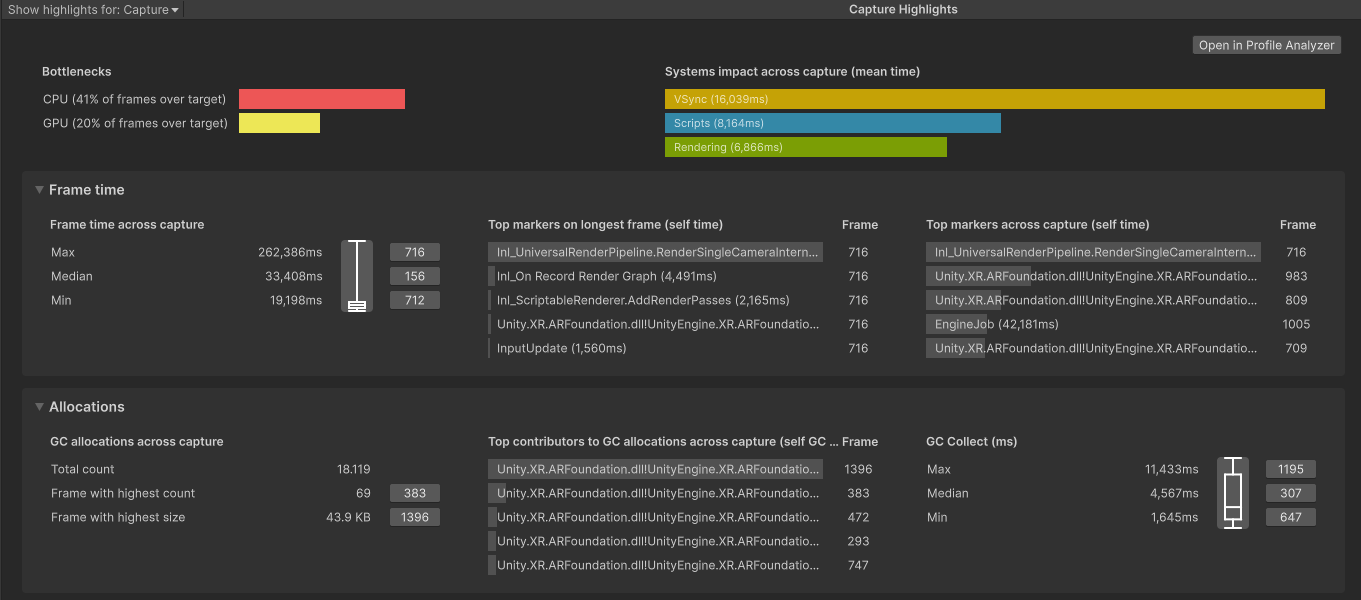
\includegraphics[width=0.7\textwidth]{images/app/HighLightsCapture.png} 
        \caption{Scheda \textit{Capture Highlights} dell'Unity Profiler.}
        \label{fig:highlightscapture}
\end{figure}

Le schede \textit{Selection Highlights} (SH, Figura~\ref{fig:highlightsselection}), relative al singolo frame selezionato, e \textit{Capture Highlights} (CH, Figura~\ref{fig:highlightscapture}), che offrono una panoramica statistica dell'intera sessione, riportano le seguenti metriche:

\begin{itemize}
\item \textbf{Utilizzo del Main Thread (SH):} attivo per il $99\%$ del tempo, con solo l'$1\%$ in attesa (\textit{Waiting}). Il dato è riferito al frame selezionato e potrebbe includere parte dei tempi di attesa di sincronizzazione (ad esempio il VSync).

\item \textbf{Impatto dei sistemi nel frame (SH):} \textit{Scripts} $13.795\text{ ms}$, \textit{GarbageCollector} $9.384\text{ ms}$, \textit{Rendering} $6.236\text{ ms}$.

\item \textbf{Colli di Bottiglia (CH):} il $41\%$ dei frame dell'intera cattura ha un tempo di CPU oltre il budget ($16.67\text{ ms}$; il frame time totale, invece, lo supera in ogni frame), mentre la GPU lo supera nel $20\%$ dei casi.

\item \textbf{Distribuzione del Frame Time (CH):} minimo $19.198\text{ ms}$ (frame $712$); mediana $33.408\text{ ms}$ (frame $156$), pari a circa $29.9\text{ FPS}$ e rappresentativa della frequenza tipica dell'applicazione; massimo $262.386\text{ ms}$, registrato al frame $716$, equivalente ad un blocco visibile di oltre un quarto di secondo. In questo frame il marker con il maggior tempo proprio (\textit{self time}, definito più sotto) è il rendering della camera della URP (\texttt{UniversalRender\allowbreak Pipeline.\allowbreak RenderSingle\allowbreak Camera\allowbreak Internal}) e non il Garbage Collector.

\item \textbf{Self Time (SH e CH):} misura il tempo netto speso in una funzione, escluse le sotto-funzioni chiamate. I principali contributi nel frame $808$ sono:
\begin{enumerate}
    \item \texttt{GC.Collect}: raccolta dei rifiuti sul Managed Heap, principale fattore di degrado temporaneo. Nel frame analizzato assorbe $9.290\text{ ms}$ ($\approx 28\%$ del tempo di frame), circa il doppio della mediana delle raccolte della cattura ($4.567\text{ ms}$); sull'intera sessione il massimo raggiunge $11.433\text{ ms}$.
    \item \texttt{Gfx.PresentFrame}: richiesta al sistema operativo e al display di mostrare il frame renderizzato. Assorbe $5.192\text{ ms}$, probabilmente legati alla sincronizzazione della presentazione (es. attesa del VSync).
    \item Routine AR Foundation (\texttt{ARSession} e \texttt{ARCameraManager}): $7.179\text{ ms}$ complessivi per l'elaborazione dei flussi video e dei sensori di tracciamento.
\end{enumerate}

\item \textbf{Mean Time (CH):} tempo medio occupato dai sistemi; i più rilevanti sono:
 \begin{itemize}
     \item \textbf{\texttt{VSync}} ($16.039\text{ ms}$): tecnologia che previene lo \textit{screen tearing} (la comparsa contemporanea di porzioni di fotogrammi diversi, visibile come interruzione orizzontale), obbligando la scheda grafica ad attendere il termine del ciclo di aggiornamento del display prima di inviare il fotogramma successivo. Nel profiler è tempo di attesa, non di lavoro.
     \item \textbf{\texttt{Scripts}} ($8.164\text{ ms}$): codice e logiche eseguite dalla CPU ad ogni frame. Un'elevata complessità ne aumenta la durata, ritardando il fotogramma successivo.
     \item \textbf{\texttt{Rendering}} ($6.866\text{ ms}$): fase in cui la CPU prepara i comandi grafici e la GPU elabora i dati geometrici e di illuminazione per generare i pixel dell'immagine; scene complesse, shader (programmi eseguiti dalla GPU per calcolare l'aspetto delle superfici) avanzati o risoluzioni elevate ne aumentano la latenza.
 \end{itemize}
In media, il lavoro effettivo (\textit{Scripts} più \textit{Rendering}, circa $15.0\text{ ms}$) rientra nel budget di $16.67\text{ ms}$, mentre la quota maggiore del frame time medio è attesa di VSync. Il frame time di circa $31\text{ ms}$ dipende quindi in larga parte dalla cadenza a $30\text{ FPS}$ e non solo dal carico computazionale; i picchi come \texttt{GC.Collect} possono invece spiegare i frame che superano il budget.
\end{itemize}

\subsection{Limiti della Sperimentazione}
I risultati vanno letti tenendo conto dei seguenti limiti:
\begin{itemize}
\item \textbf{Build di debug con Profiler collegato:} introducono un overhead aggiuntivo (il Profiler stesso occupa $36.9\text{ MB}$ di memoria); i valori assoluti sono quindi indicativi e, con ogni probabilità, peggiori rispetto a una build di rilascio.
\item \textbf{Singolo dispositivo:} i test sono stati eseguiti solo sul Motorola Edge 70, quindi i risultati non sono generalizzabili ad altri modelli o fasce di mercato.
\item \textbf{Frame selezionato:} l'analisi di dettaglio riguarda un singolo frame (il $808$), prossimo alla mediana, che non cattura la variabilità della sessione né il caso peggiore (frame $716$); per il comportamento complessivo si fa riferimento ai \textit{Capture Highlights}.
\item \textbf{Misura del tempo GPU:} il \textit{GPU Time} non è disponibile per il frame analizzato, quindi il carico grafico è stimato indirettamente.
\item \textbf{Limite alla frequenza di aggiornamento:} il tempo mediano di circa $33\text{ ms}$ potrebbe essere in parte determinato da un cap a $30\text{ FPS}$ (VSync, \texttt{Application.\allowbreak targetFrameRate} o cadenza del flusso della fotocamera) e non solo dal carico computazionale.
\end{itemize}











